\documentclass[letterpaper,12pt]{article}
\usepackage{amsmath}
\usepackage{amssymb}
\usepackage{amsthm}
\usepackage{graphicx}
%\usepackage{subfig}
\usepackage[margin=2.5cm,nohead]{geometry}

%\input{../commands}
%\setkeys{Gin}{draft=true}
%
%\newtheorem{thm}{Theorem}%[subsection]
%\newtheorem{lem}[thm]{Lemma}
%\newtheorem{cor}[thm]{Corollary}
%\newtheorem{prop}[thm]{Proposition}
%\newtheorem{remark}[thm]{Remark}
%\newtheorem*{thm*}{Theorem}
%\newtheorem*{lem*}{Lemma}



\begin{document}

\begin{center}
    {\bf UNIVERSITY OF CALIFORNIA AT BERKELEY}\\
    {\bf Department of Mechanical Engineering}\\
    {\bf ME233 Advanced Control Systems II}\\
    Spring 2016\\
\end{center}
\noindent
{\Large \bf Homework \#5 }\\[-3em]
\begin{flushright}
\begin{tabular} {lll}
    Assigned: &  Apr.\ 6 & (W) \\
    Due: & Apr.\ 12 & (Tu)
\end{tabular}
\end{flushright}

%\noindent
%\textbf{Warning:} This homework involves doing quite a bit of computer simulation. Please do not procrastinate until the last day.

\begin{enumerate}

\item
Figure~\ref{fig:Disturbance_Observer_DO} shows the feedback interconnection for a system with a disturbance observer.
\begin{figure}[h]
    \centering
    \begin{minipage}{2.5in}
        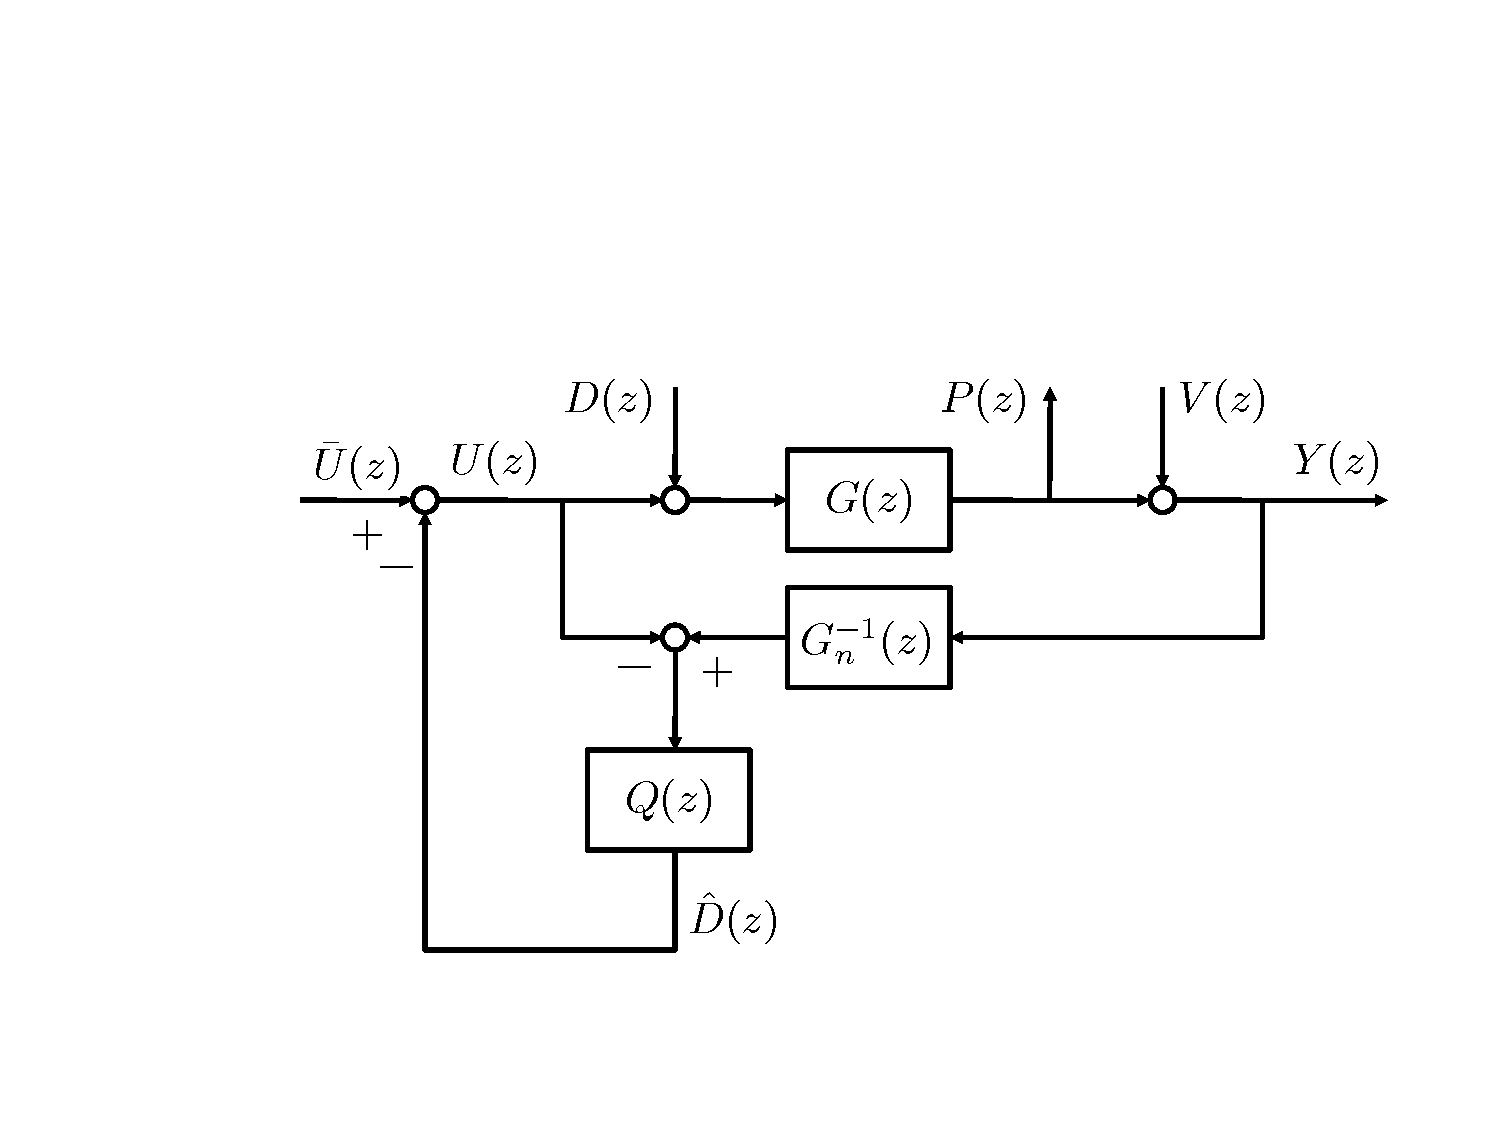
\includegraphics[width=2.5in]{Disturbance_Observer_DO}
        \caption{Disturbance Observer Structure}
        \label{fig:Disturbance_Observer_DO}
    \end{minipage}
    \qquad
    \begin{minipage}{2.5in}
        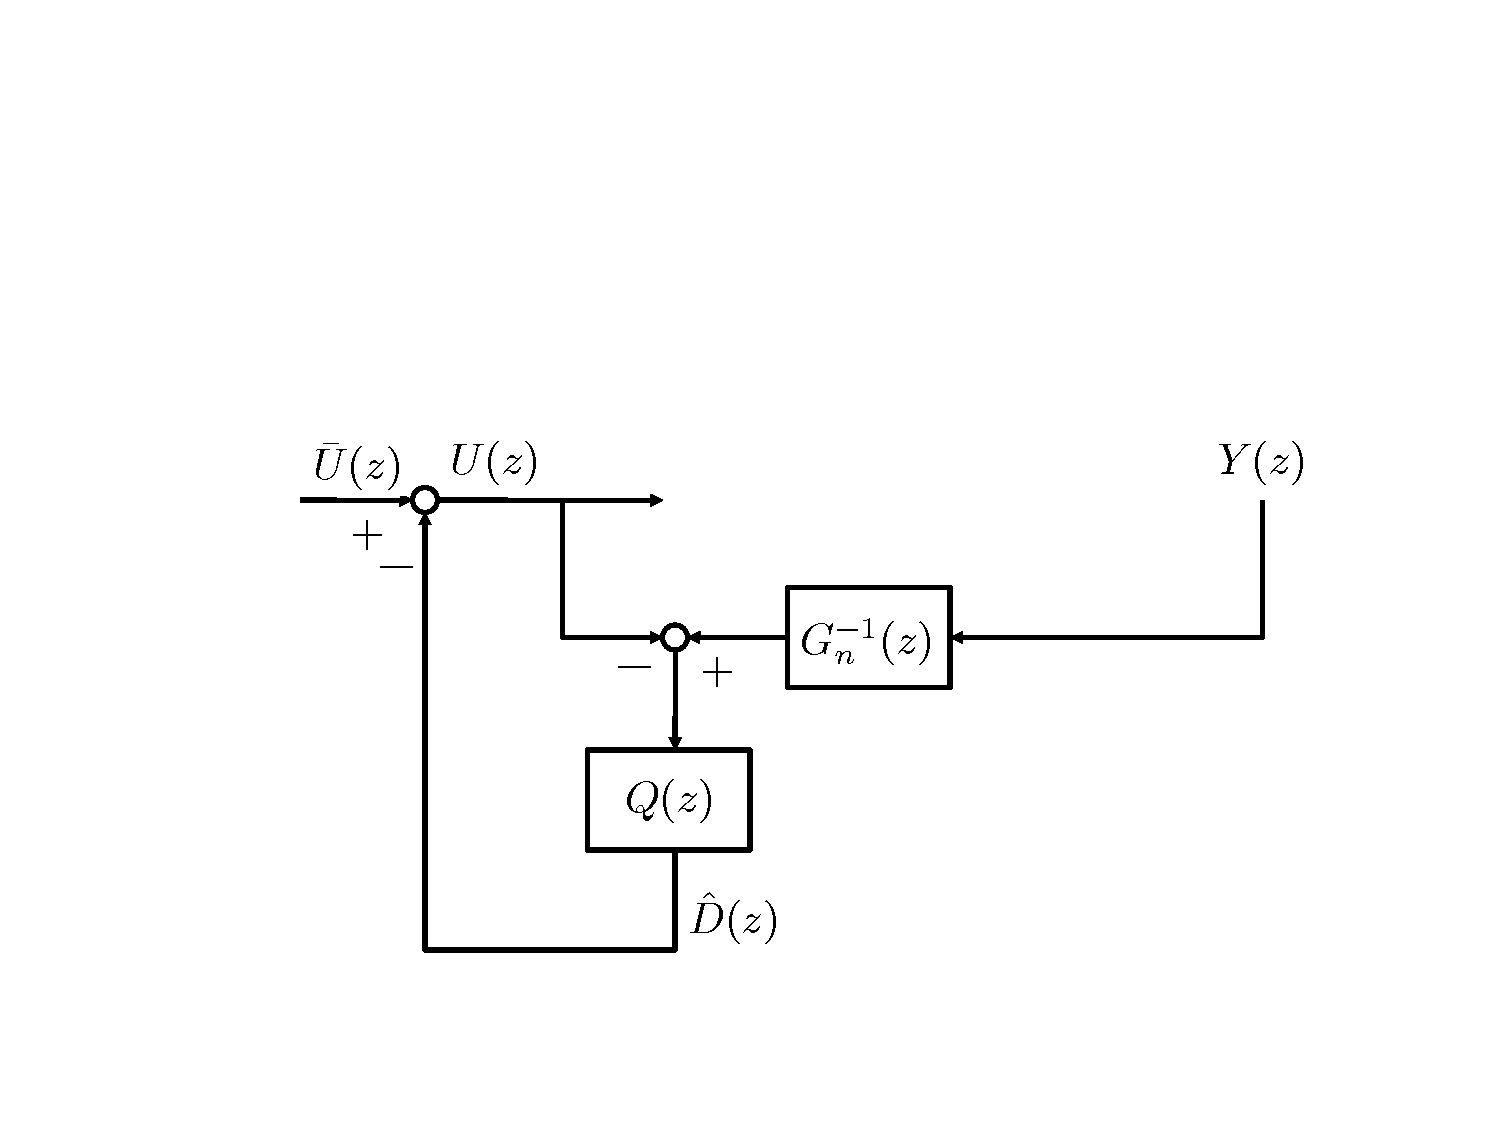
\includegraphics[width=2.5in]{Disturbance_Observer_controller}
        \caption{Disturbance Observer---Controller Only}
        \label{fig:Disturbance_Observer_controller}
    \end{minipage}
\end{figure}
When implementing the disturbance observer, we only implement the portion that generates $U(z)$ from $\bar{U}(z)$ and $Y(z)$, as shown in Fig.~\ref{fig:Disturbance_Observer_controller}.

\begin{enumerate}
    \item
    Find the transfer function from $Y(z)$ and $\bar{U}(z)$ to $U(z)$ in Fig.~\ref{fig:Disturbance_Observer_controller}.

    \item
    Suppose that $G_n^{-1}$ is proper. In this case, it is valid to choose $Q(z) = \alpha \in \mathcal{R}$. Based on your answer from the previous part, note that the block diagram in Fig.~\ref{fig:Disturbance_Observer_controller} is not well-posed when $\alpha = 1$. Does there exist $\alpha \in \mathcal{R}$ such that the closed-loop transfer function from $D(z)$ to $P(z)$ is zero? If not, is there a limit to how small we can make the transfer function from $D(z)$ to $P(z)$?

%    How should $\alpha$ be chosen when the primary control objective is disturbance rejection (i.e.\ if you neglect sensor noise and stability robustness)?
\end{enumerate}



\newpage
\item
%from 2010, HW10, p2
Consider the feedback system in Fig. \ref{pole-placement-feedback-loop}
\begin{figure}[h]
    \centering
    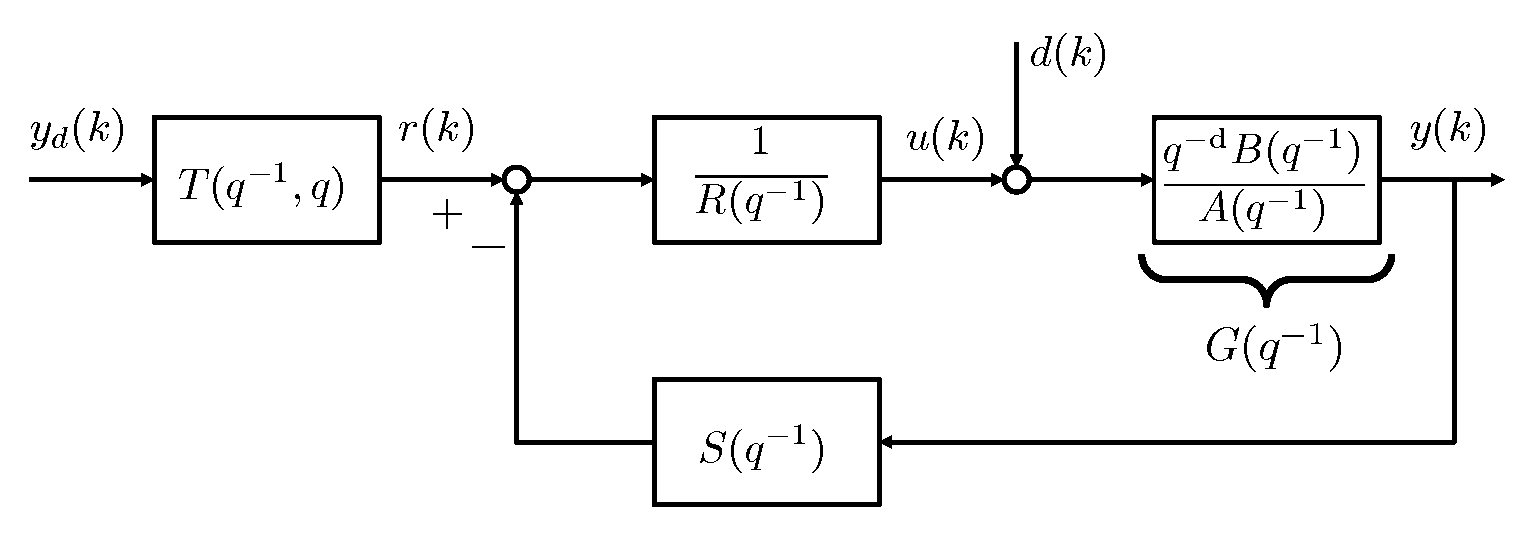
\includegraphics[width=4.5in]{pole-placement-feedback-loop-yd}
    \caption{Feedback System}
    \label{pole-placement-feedback-loop}
\end{figure}
where $u(k)$ and $d(k)$ are respectively the control and disturbance plant inputs, $y_d(k)$ is the reference model's output, and $r(k)$ is the reference input to the feedback block.

The control objective is to reject the persistent deterministic disturbance $d(k)$, place the feedback closed-loop poles, and  track the desired output $y_d(k)$.

%In order to help you verify your solutions of the Diophantine equation (also known as the Bezout equation), I have uploaded the MATLAB file bezout.m, which solves this equation. However, I advise you to solve the Diophantine equations in this problem by hand, so that you gain an understanding of what is involved in the solution of this type of equation.

\begin{enumerate}
    \item
    The plant transfer function $G(z)$ is derived from a continuous time transfer function $G(s)$ that is preceded by a zero-order hold and followed by a sampler, and is given by
    \begin{align*}
        G(z) = \frac{\bar{B}(z)}{\bar{A}(z)}
            = (1 - z^{-1}) \, {\cal Z} \left \{ {\cal L}^{-1} \left ( \frac{G(s)}{s} \right ) \right \}\,,
    \end{align*}
    where
    \begin{align*}
        G(s) = \frac{1}{s(s + 1)}
    \end{align*}
    and the sampling time is $T = 0.5$ seconds.

    Calculate the plant polynomials $A(q^{-1}) = 1 + a_1 q^{-1} + a_2 q^{-2}$,  $B(q^{-1}) = b_o +  b_1 q^{-1}$  and pure delay time $\textrm{d}$. %You can use the MATLAB function {\tt c2d} for this purpose.\\

    \item
    \label{sec:track}
    The tracking control objective is to follow the reference signal $y_d(k)$, which is the output of the reference model
    \begin{align}
        A_m (q^{-1}) y_d(k) = q^{-\textrm{d}} B_m(q^{-1}) u_d(k) \,.
        \label{eq:yd_def}
    \end{align}
    Select the coefficients of the second order polynomial $A_m(q^{-1}) = 1 + a_{m1}\, q^{-1} + a_{m2} \, q^{-2}$, so that the reference model has a natural frequency of 1 rad/sec and a damping ratio of 0.707.

    \textbf{Hint:} Remember that, since $z = e^{s T}$, we can calculate the discrete time poles by $p_d = e^{p_c \, T}$, where $p_d$ is the discrete time pole, $p_c$ is the continuous time pole and $T$ is the sampling time.

    \item
    Letting $B_m(q^{-1}) = b_{mo}$, select $b_{mo}$ so that the reference model has unity static gain
    \footnote{i.e. if $\lim_{k \to \infty} u_d(k)  = u_{ss}$  then  $\lim_{k \to \infty} y_d(k)  = u_{ss}$.}.

    \item
    Choose the coefficients of the closed-loop system characteristic polynomial (after pole-zero cancelation)
    \begin{align*}
        A_c^{' } (q^{-1}) =  1 + a^{'}_{c1}\, q^{-1} + a^{'}_{c2} \, q^{-2}
    \end{align*}
    so that the closed-loop feedback dynamics from $r(k)$ to $y(k)$ behaves as a second-order system with  a natural frequency of 2 rad/sec and a damping ratio of 0.5.

    \item
    \label{sec:p4}
    Design the control system under the following specifications and assumptions:
    \begin{enumerate}
        \item
        The closed-loop system characteristic polynomial (before pole-zero cancelation) is given by
        \begin{align*}
            A_c (q^{-1}) = A_c^{' } (q^{-1})  B^s(q^{-1})
        \end{align*}
        where
        \begin{align*}
            B^s(q^{-1}) & = \frac{1}{b_o} B(q^{-1}),
                & B^u(q^{-1}) & = b_o\,,
        \end{align*}
        and $b_o$ is the leading coefficient of $B(q^{-1})$. This means that all of the plant zeros will be canceled by the feedback system.

        \item
        Assume that
        $d(k) = 0$. This means that the disturbance annihilating polynomial is selected to be $A_d(q^{-1}) = 1$.

        \item
        The feedforward compensator  $T(q^{-1},q)$ must be selected so that perfect tracking is achieved under a zero initial state for both the plant and the reference model.
    \end{enumerate}

    \item
    \label{sec:p5}
    Do a computer simulation of the control system designed in problem \ref{sec:p4} when $y_d(-1) = y_d(0) = y(-1) = y(0) = 0$ and
    \begin{align}
        u_d(k) & = \left [ u_s(k) - 2\,u_s(k - 25)  \right ]
            + \, \left [ 2\,u_s(k - 50) - 2\,u_s(k - 75)  \right ]
            \label{eq:uc_def} \\
        %\cdots +
        %\, \left [ u_s(k - n 50) - u_s(k - (n 50 + 25))  \right ]
        d(k) & = 0.5 u_s(k-40)
            \label{eq:d_def}
    \end{align}
    where $u_s(j)$ is the unit step function, i.e.\
    \begin{align*}
        u_s(j) = \left \{ \begin{array}{ccc}
                0 & \hspace{1em} & j < 0\\
                1 & \hspace{1em} & j \ge 0
            \end{array} \right .
    \end{align*}
    Plot $u_d(k)$, $y_d(k)$, $y(k)$ and $u(k)$.

    \item
    \label{sec:p6}
    Design the control system under the same specifications in problem \ref{sec:p4}, except that assume now that $d(k) = d(k-1)$.

    \item
    Do a computer simulation of the control system designed in problem \ref{sec:p6} under the  conditions
    described in problem \ref{sec:p5}. Plot $u_d(k)$, $y_d(k)$, $y(k)$ and $u(k)$.

    \item
    \label{sec:p8}
    Design the control system under the following specifications and assumptions:

    \begin{enumerate}
        \item
        The closed loop  system characteristic polynomial satisfies
        \begin{align*}
            A_c (q^{-1}) &= A_c^{' } (q^{-1})  B^s(q^{-1})
        \end{align*}
        where
        \begin{align*}
            B^s(q^{-1}) & = 1,
                & B^u(q^{-1}) & = B(q^{-1})\,,
        \end{align*}
        This means that none of the plant zeros will be canceled by the feedback system.

        \item
        Assume that
        $d(k) = d(k-1)$.

        \item
        The feedforward compensator  $T(q^{-1},q)$ is designed using the zero-phase error tracking control approach.
    \end{enumerate}

    \item
    Do a computer simulation of the control system designed in problem \ref{sec:p8} under the  conditions
    described in problem \ref{sec:p5}. Plot $u_d(k)$, $y_d(k)$, $y(k)$ and $u(k)$.

    \item
    Discuss the outcome of the simulation results. In particular
    \begin{itemize}
        \item Comment on the effectiveness of the zero-phase feedforward control technique.
        \item Compare the control effort $u(k)$ when the zeros are canceled vs when the zeros are not canceled.
    \end{itemize}
\end{enumerate}

%\newpage
%\input{hw7p3}

\end{enumerate}


\end{document}


